\section{Proposed System Block Diagram}
As explained in the preceding section, the two parts of the system, \gls{rtls} ans its implementation can be explained through the Figure \ref{fig:BlockDiagram}.

\begin{figure}[htpb]
\centering
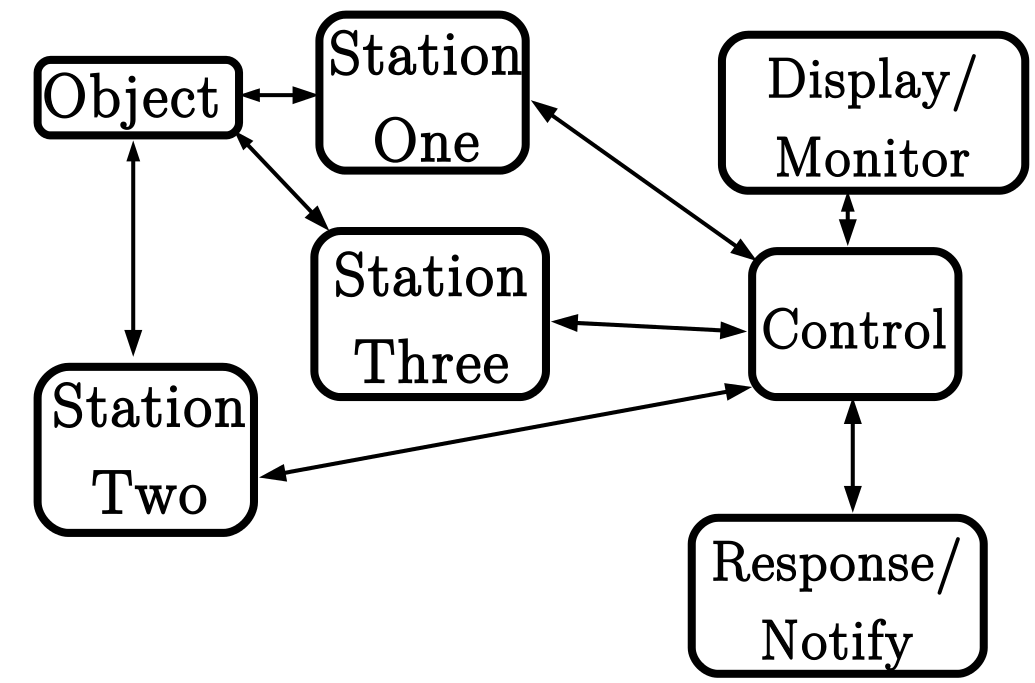
\includegraphics[scale=.34]{./Images/BlockDiagram.png}
\caption{System Block Diagram}
\label{fig:BlockDiagram}
\end{figure}

The object to be tracked is equipped with a transceiver that can independently communicate with the three stations around it in the field of it. The distance can be measured with procedure possibly time of flight. The distance obtained is then fed to the control unit from each of the three stations. Then the data is sent to the computer for analysis using a microcontroller. The computer analyses the data, stores them and then gives out the necessary signal to the user through the use of any of the signaling method -  light or sound or any convenient method.
